\item \textbf{Hold out the last 3 months of 2017 for out-of-sample prediction and implement the following:} 
\begin{enumerate}
\item \textbf{Begin by forecasting with a single LSTM-layer and optimize its performance by varying the various hyper-parameters, for example: LSTM units, no. of layers, batch  size, learning  rate, etc. Plot and analyze the model performance (accuracy and loss) vs. the number of epochs. You should also test different  techniques to avoid model overfitting. Be sure to include and  contrast examples of the different approaches – don’t only show “the best”. Plot the predictions and report the forecasting error using appropriate metrics.}
\item \textbf{Repeat the forecasting using a 1D CNN-based  forecasting model. Evaluate and optimize its performance similar to point part (a). This may require you to go beyond course material, but there are plenty of resources online that you can leverage.}
\item \textbf{Now, implement a hybrid ConvLSTM forecasting model by combining the CNNs and LSTMs together. Evaluate and optimize its performance in comparison to part (a) and (b). Plot the predictions and report the forecasting error using appropriate metrics in comparison to part (a) and (b).}
\end{enumerate}

\textit{Figure \ref{fig:ass4_frameworks} depicts my framework for all three parts of this assignment. For each part, we used the same procedure but with different architectures for DNN. In the following, I will discuss each step.  }

\begin{figure}[H]
    \centering
    \begin{minipage}[b]{1.1\textwidth}
        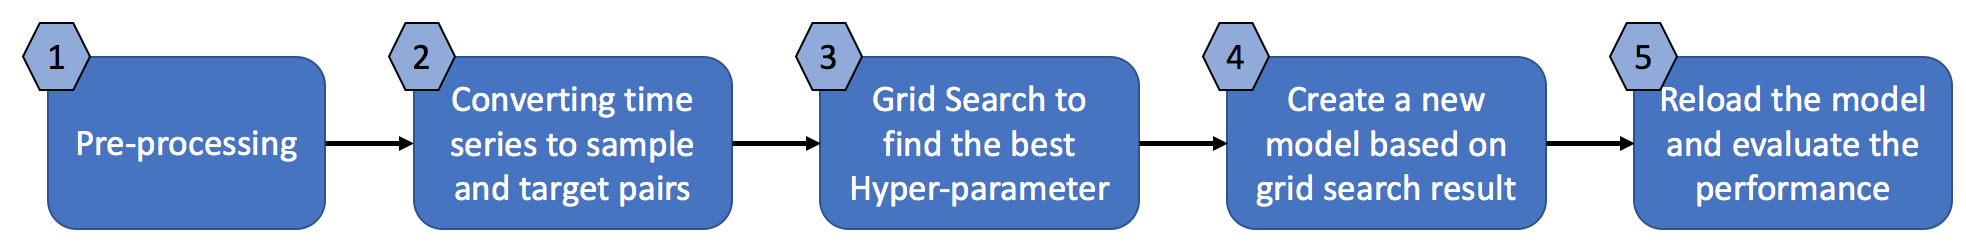
\includegraphics[width=\textwidth]{manuscript/src/figures/Ass4/Ass4_frameworks.png}
    \end{minipage}
    \caption{The framework that was used for this question.}
    \label{fig:ass4_frameworks}
\end{figure}


\textit{In the pre-processing step, we used the last 50 samples for the test and others for the training set. This part is equal to the last three months. Then the MinMax function was used to change the input scaling between zero and one due to the fact that the signal range was large. for this purpose, I used the training set for finding min and max values and then transformed both training and test set based on these two values. Figure \ref{fig:Ass4_Q2a_raw_signal} shows the raw data used for this project.}

\begin{figure}[H]
    \centering
    \begin{minipage}[b]{1\textwidth}
        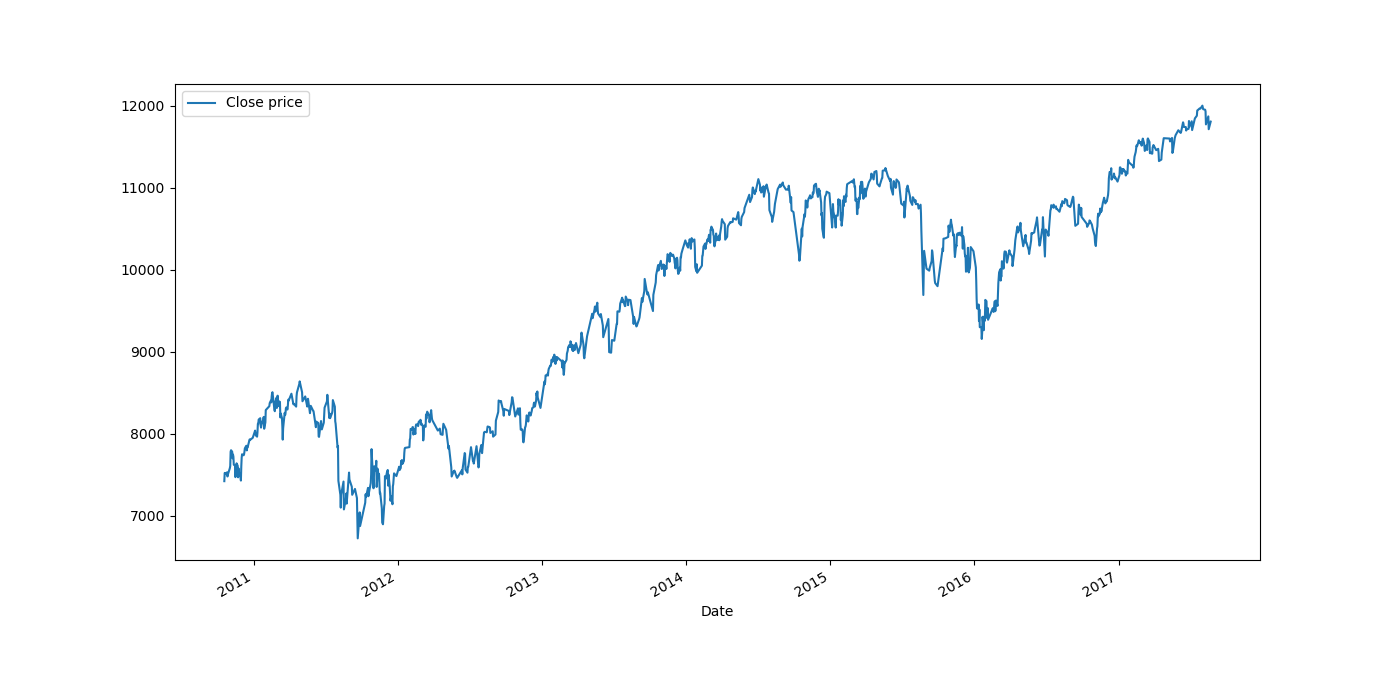
\includegraphics[width=\textwidth]{manuscript/src/figures/Ass4/Ass4_Q2a_raw_signal.png}
    \end{minipage}
    \caption{The raw signal.}
    \label{fig:Ass4_Q2a_raw_signal}
\end{figure}

\textit{In the next step, I have converted normalized time-series data to pairs samples and output, or in other words, the supervised data. For doing this, I have used the create\_dataset() function from the tutorial code. This function needs two arguments time-series signal and window size and returns a sequence of a signal based on window size as input, and then the next value as output. The below image depicts this converting with the window size of 3. For this question, the window size is set to 15.}

\begin{figure}[H]
     \centering
     \begin{subfigure}[b]{0.55\textwidth}
         \centering
         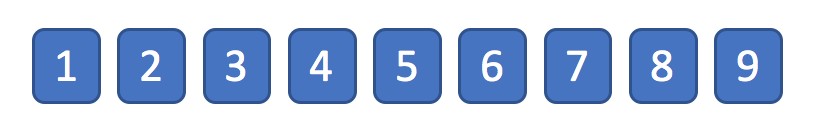
\includegraphics[width=1\textwidth]{manuscript/src/figures/Ass4/time.png}
         \caption{The time-series signal.}
         \label{fig:ROC_all}
     \end{subfigure}
     \vfill
     \begin{subfigure}[b]{.25\textwidth}
         \centering
         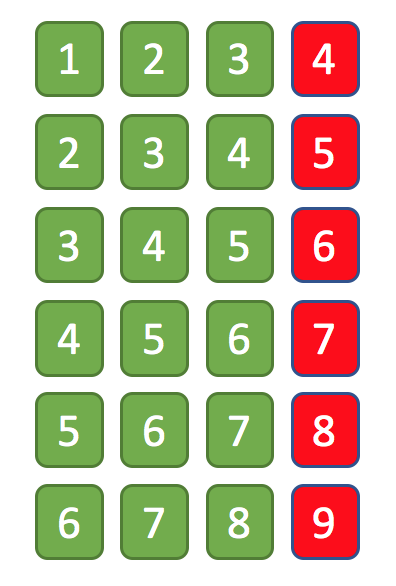
\includegraphics[width=1\textwidth]{manuscript/src/figures/Ass4/sup.png}
         \caption{Samples sequence with corresponding output values.}
         \label{fig:ROC_fcn}
     \end{subfigure} 
        \caption{Converting time-series signal to the supervised data. For this example, window size is equal to 3. }
        \label{fig:ROC}
\end{figure}

\textit{To optimize our model, I have used grid search to find the best hyperparameters. Since grid search is a function on the Scikit-learn library, we needed to convert the Keras model to a Scikit-learn model. So that I have imported KerasClassifier from "keras.wrappers.scikit\_learn". Then a GridSearchCV instance was made based on our model, the search space, and a 5-fold cross-validation object. Tables \ref{tab:Ass4_Q2a} to \ref{tab:Ass4_Q2c} show the search space of grid search as well as the best hyper-parameters for our model for all three parts of this question.}


\begin{table}[H]
\centering
\caption{The search space of GridSearchCV method as well as the best hyper-parameters for part (a).}
\label{tab:Ass4_Q2a}
\begin{lstlisting}
param_grid=
    {
        'LSTM_units':       [5, 15, 10],
        'batch_size':       [16, 32, 64],
        'learning_rate':    [0.0001, 0.001, 0.01]
    }

Best hyper-parameters=
    {
        'LSTM_units':       10,
        'batch_size':       16, 
        'learning_rate':    0.01
     }
\end{lstlisting}



\end{table}

\begin{table}[H]
\centering
\caption{The search space of GridSearchCV method as well as the best hyper-parameters for part (b).}
\label{tab:Ass4_Q2b}
\begin{lstlisting}
param_grid=
    {
        'batch_size':       [16, 32, 64],
        'learning_rate':    [0.0001, 0.001, 0.01]
    }

Best hyper-parameters=
    {
        'batch_size':       16, 
        'learning_rate':    0.01
     }
\end{lstlisting}
\end{table}


\begin{table}[H]
\centering
\caption{The search space of GridSearchCV method as well as the best hyper-parameters for part (c).}
\label{tab:Ass4_Q2c}
\begin{lstlisting}
param_grid=
    {
        'batch_size':       [16, 32, 64],
        'learning_rate':    [0.0001, 0.001, 0.01]
    }

Best hyper-parameters=
    {
        'batch_size':       64, 
        'learning_rate':    0.01
     }
\end{lstlisting}

\end{table}

 

\textit{After optimizing hyperparameters, a new model has been created according to the best hyperparameters of the last step. Then the model was trained with 100 epochs. Also, validation\_split was set to 0.2 which means 20 percent of the training data to be used as validation data. Validation data was used for avoiding the overfitting problem. Moreover, a callback method was used to track the loss function on the training and validation set. The callback is called only in the training phase with the model.fit() function to save the best model in a checkpoint file, so the model could be loaded later. Tables \ref{tab:Ass4_Q2a_result} to  \ref{tab:Ass4_Q2c_result} indicate the results of overtrained and trained models on the test and train set. }


\begin{table}[H]
\centering
\caption{The results of overtrained and trained models on the test and train set for part (a).}
\label{tab:Ass4_Q2a_result}
\begin{tabular}{lr}
\toprule
{} & RMSE\\
\midrule
Overtrained model on Train set: & 105.94 \\
Trained model on Train set: & 106.13 \\
Overtrained model on Test set: & 142.18  \\
Trained model on Test set:  & 82.33 \\

\bottomrule
\end{tabular}



\end{table}

\begin{table}[H]
\centering
\caption{The results of overtrained and trained models on the test and train set for part (b).}
\label{tab:Ass4_Q2b_result}
\begin{tabular}{lr}
\toprule
{} & RMSE\\
\midrule
Overtrained model on Train set: & 125.88 \\
Trained model on Train set: & 110.47 \\
Overtrained model on Test set: & 314.87 \\
Trained model on Test set:  & 117.64 \\

\bottomrule
\end{tabular}



\end{table}


\begin{table}[H]
\centering
\caption{The results of overtrained and trained models on the test and train set for part (c).}
\label{tab:Ass4_Q2c_result}
\begin{tabular}{lr}
\toprule
{} & RMSE\\
\midrule
Overtrained model on Train set: & 121.36 \\
Trained model on Train set: & 117.86 \\
Overtrained model on Test set: & 600.56 \\
Trained model on Test set:  & 318.32 \\

\bottomrule
\end{tabular}


\end{table}





\textit{For part (a), an LSTM model was built. Figure \ref{fig:modela} indicates the layers of this model. Figures \ref{fig:Ass4_Q2a_forcasted} and \ref{fig:Ass4_Q2a_Training} show the predicted output and Training and Validation Loss, respectively.}


\begin{figure}[H]
    \centering
    \begin{minipage}[b]{0.5\textwidth}
        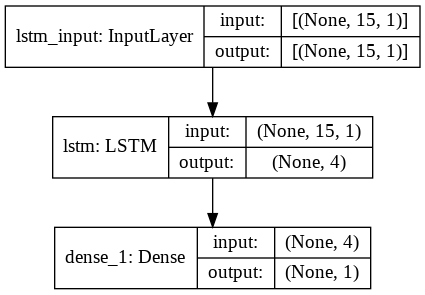
\includegraphics[width=\textwidth]{manuscript/src/figures/Ass4/a2.png}
    \end{minipage}
    \caption{The graph of model used in part (a).}
    \label{fig:modela}
\end{figure}

\begin{figure}[H]
    \centering
    \begin{minipage}[b]{1\textwidth}
        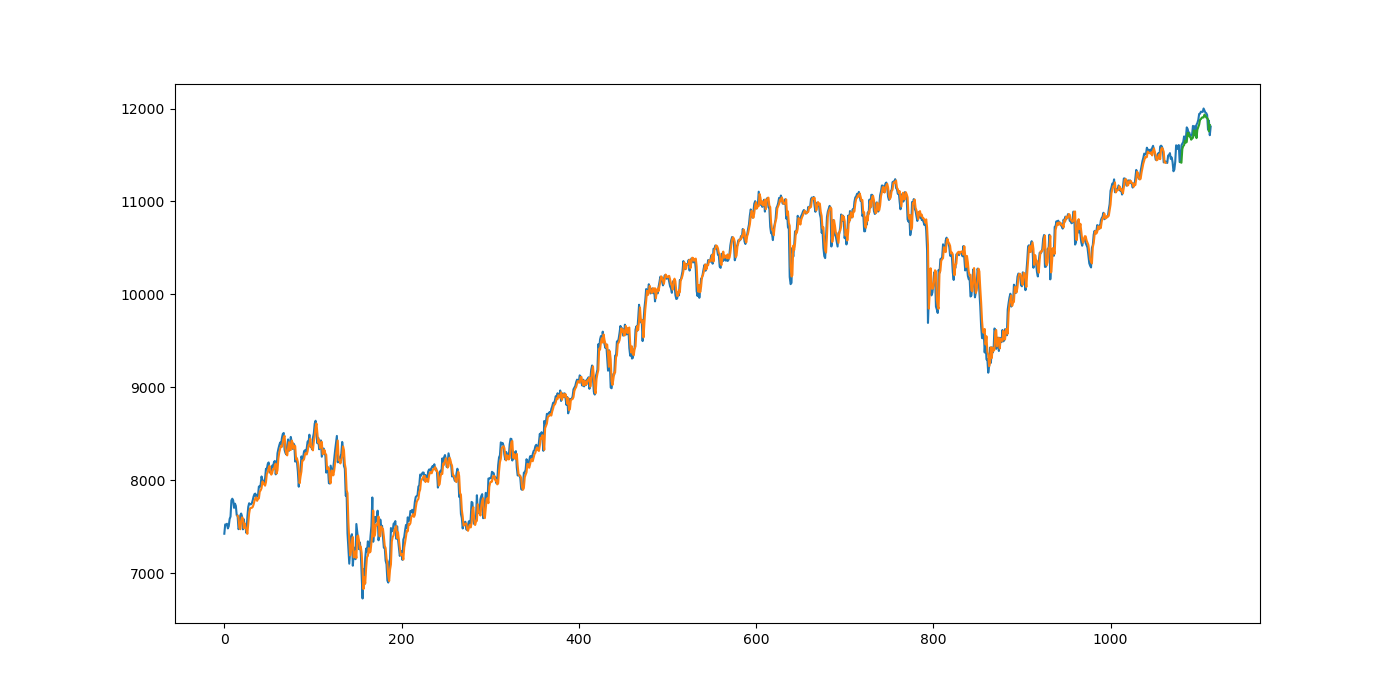
\includegraphics[width=\textwidth]{manuscript/src/figures/Ass4/Ass4_Q2a_forcasted.png}
    \end{minipage}
    \caption{The original signal and predicted value of model (a).}
    \label{fig:Ass4_Q2a_forcasted}
\end{figure}

\begin{figure}[H]
    \centering
    \begin{minipage}[b]{1\textwidth}
        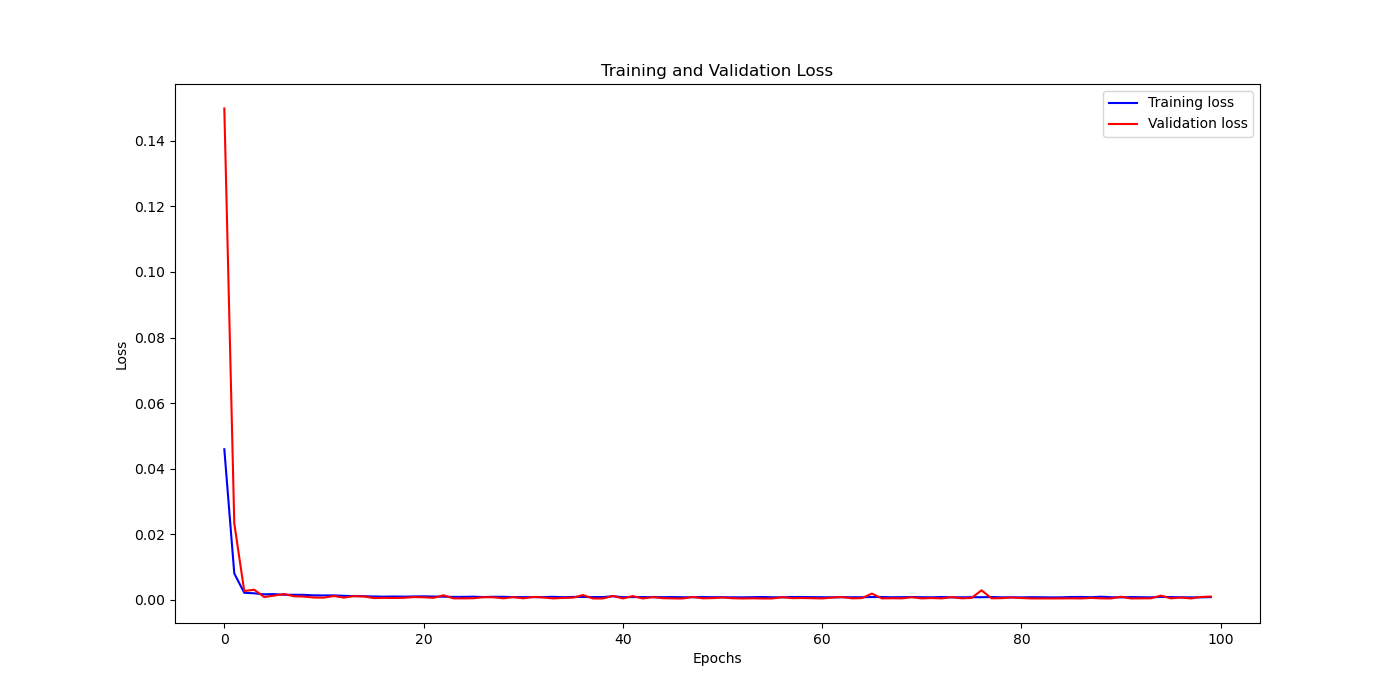
\includegraphics[width=\textwidth]{manuscript/src/figures/Ass4/Ass4_Q2a_Training and Validation Loss.png}
    \end{minipage}
    \caption{Training and Validation Loss of model (a) versus epoch.}
    \label{fig:Ass4_Q2a_Training}
\end{figure}














\textit{For part (b), Fully Convolutional Networks (FCN) \cite{WangTimeBaseline} has been implemented. This model is an end-to-end convolutional network with three blocks. Each block has a convolutional layer followed by batch normalization and ReLU activation layer (see figure \ref{fig:modelb}). The output of the third block is averaged over the time dimension which corresponds to the global average pooling (GAP) layer. Finally, a dense layer is fully connected to the GAP layer’s output to produce the final prediction. Figures \ref{fig:Ass4_Q2b_forcasted} and \ref{fig:Ass4_Q2b_Training} show the predicted output and Training and Validation Loss, respectively. }

\begin{figure}[H]
    \centering
    \begin{minipage}[b]{0.6\textwidth}
        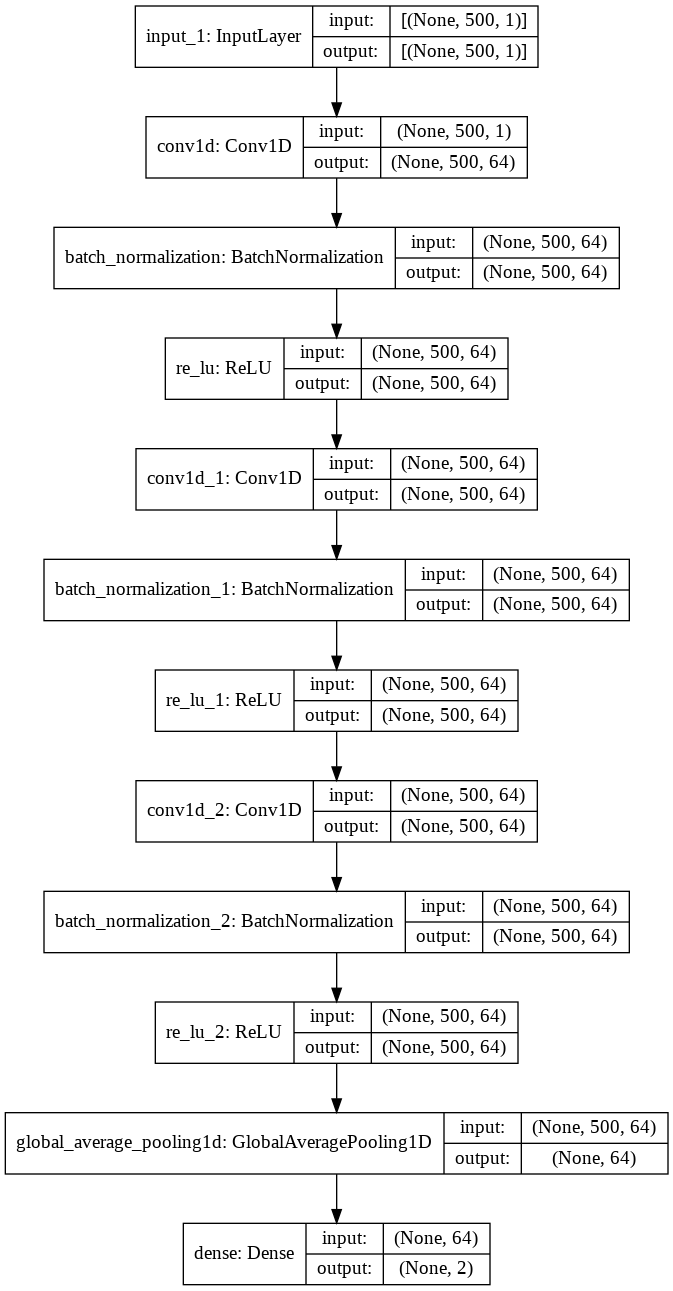
\includegraphics[width=\textwidth]{manuscript/src/figures/Ass4/b2.png}
    \end{minipage}
    \caption{The graph of model used in part (b).}
    \label{fig:modelb}
\end{figure}

\begin{figure}[H]
    \centering
    \begin{minipage}[b]{1\textwidth}
        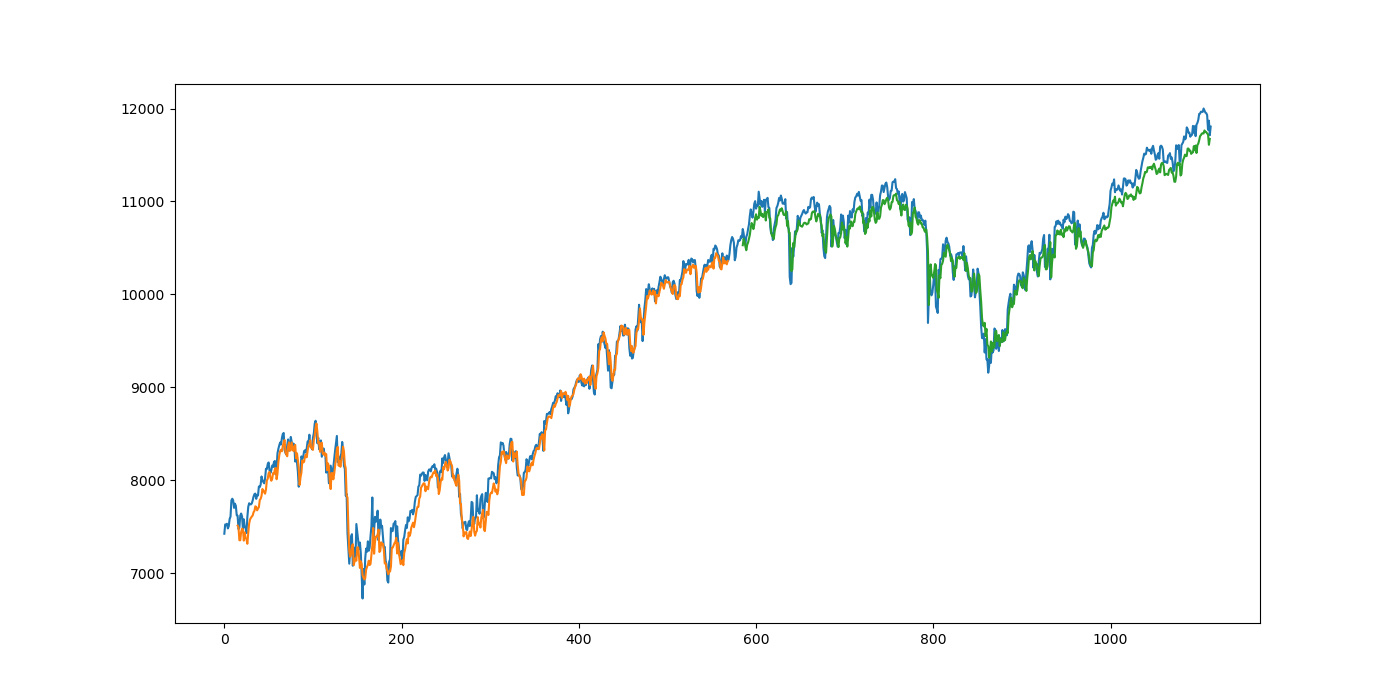
\includegraphics[width=\textwidth]{manuscript/src/figures/Ass4/Ass4_Q2b_forcasted.png}
    \end{minipage}
    \caption{The original signal and predicted output of model (b).}
    \label{fig:Ass4_Q2b_forcasted}
\end{figure}

\begin{figure}[H]
    \centering
    \begin{minipage}[b]{1\textwidth}
        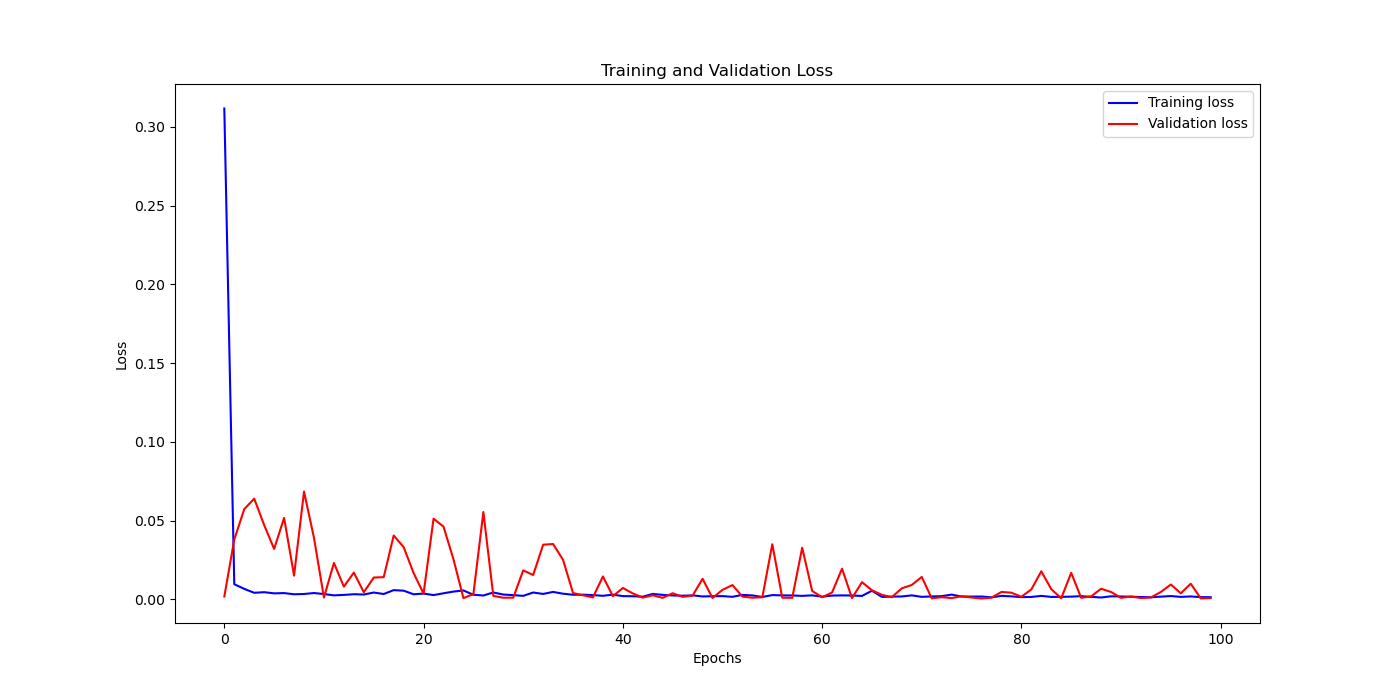
\includegraphics[width=\textwidth]{manuscript/src/figures/Ass4/Ass4_Q2b_Training and Validation Loss.png}
    \end{minipage}
    \caption{Training and Validation Loss of model (b) versus epoch.}
    \label{fig:Ass4_Q2b_Training}
\end{figure}















\textit{For part (c), since Keras library does not support the ConvLSTM1D, a CNN-LSTM model was implemented (I talked about it with Pradeep). For building this model, I have used Fully Convolutional Networks (FCN) in a Sequence and then replaced the GAP layer with an LSTM layer (see figure \ref{fig:modelc}). Figures \ref{fig:Ass4_Q2c_forcasted} and \ref{fig:Ass4_Q2c_Training} show the predicted output and Training and Validation Loss, respectively.}

\begin{figure}[H]
    \centering
    \begin{minipage}[b]{0.6\textwidth}
        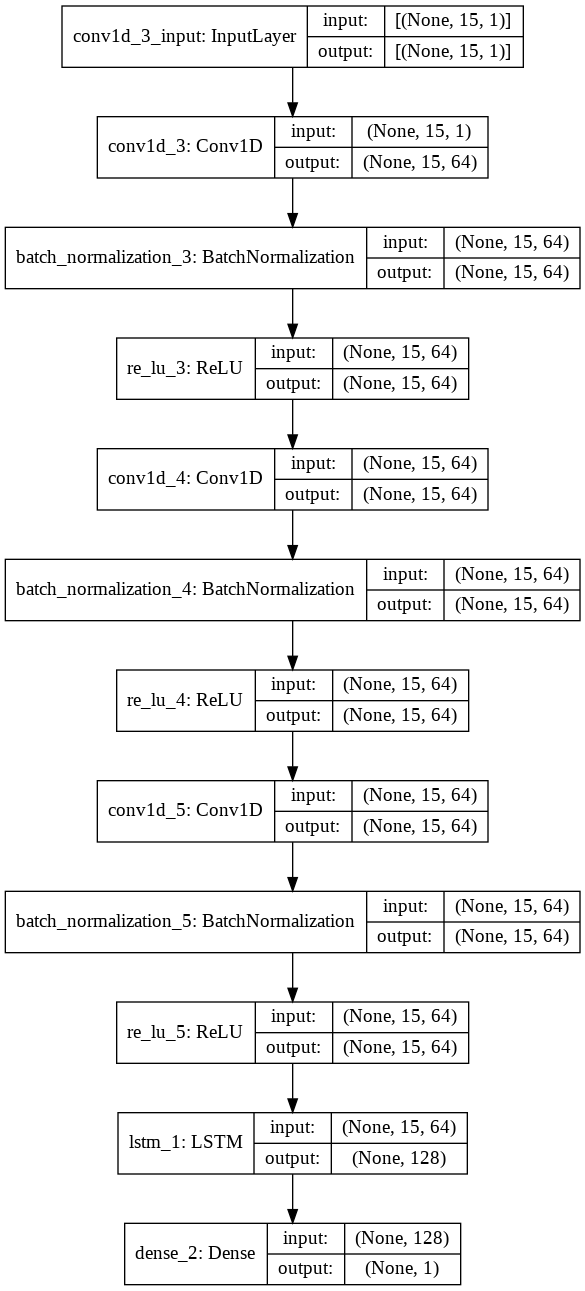
\includegraphics[width=\textwidth]{manuscript/src/figures/Ass4/c2.png}
    \end{minipage}
    \caption{The graph of model used in part (c).}
    \label{fig:modelc}
\end{figure}





\begin{figure}[H]
    \centering
    \begin{minipage}[b]{1\textwidth}
        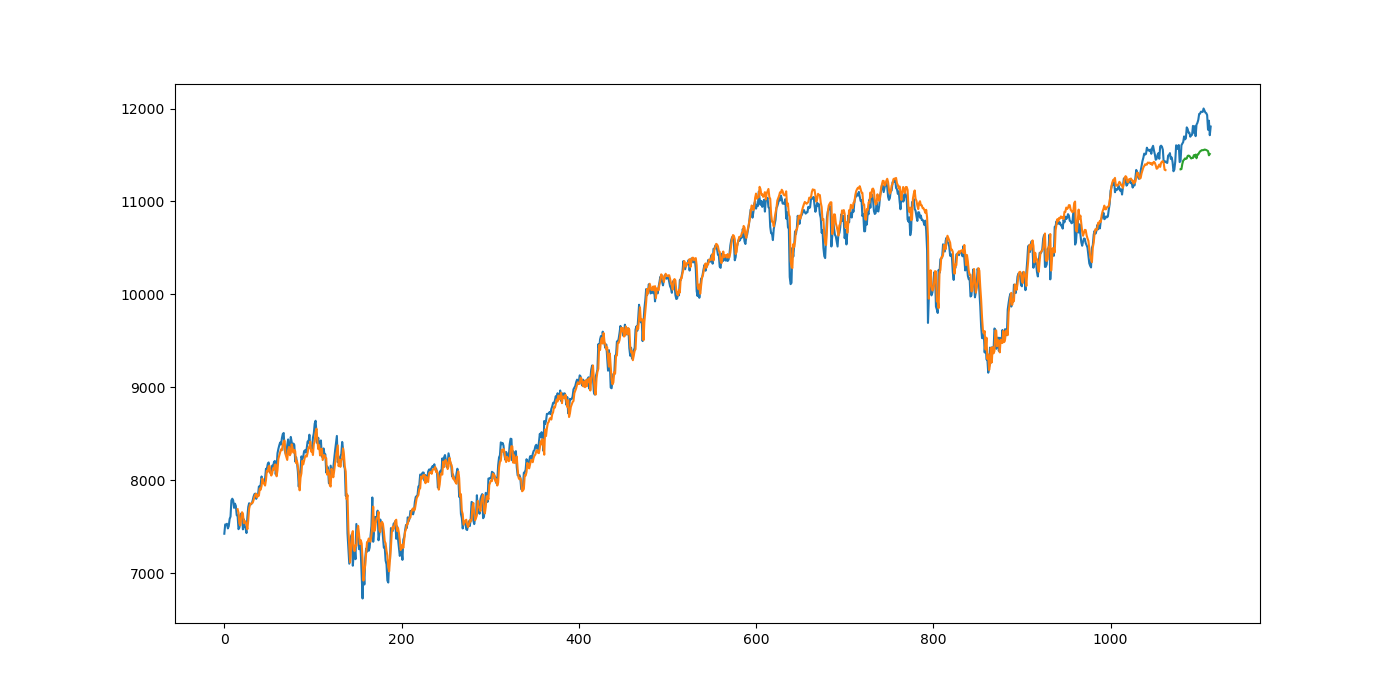
\includegraphics[width=\textwidth]{manuscript/src/figures/Ass4/Ass4_Q2c_forcasted.png}
    \end{minipage}
    \caption{The original signal and predicted output of model (b).}
    \label{fig:Ass4_Q2c_forcasted}
\end{figure}






\begin{figure}[H]
    \centering
    \begin{minipage}[b]{1\textwidth}
        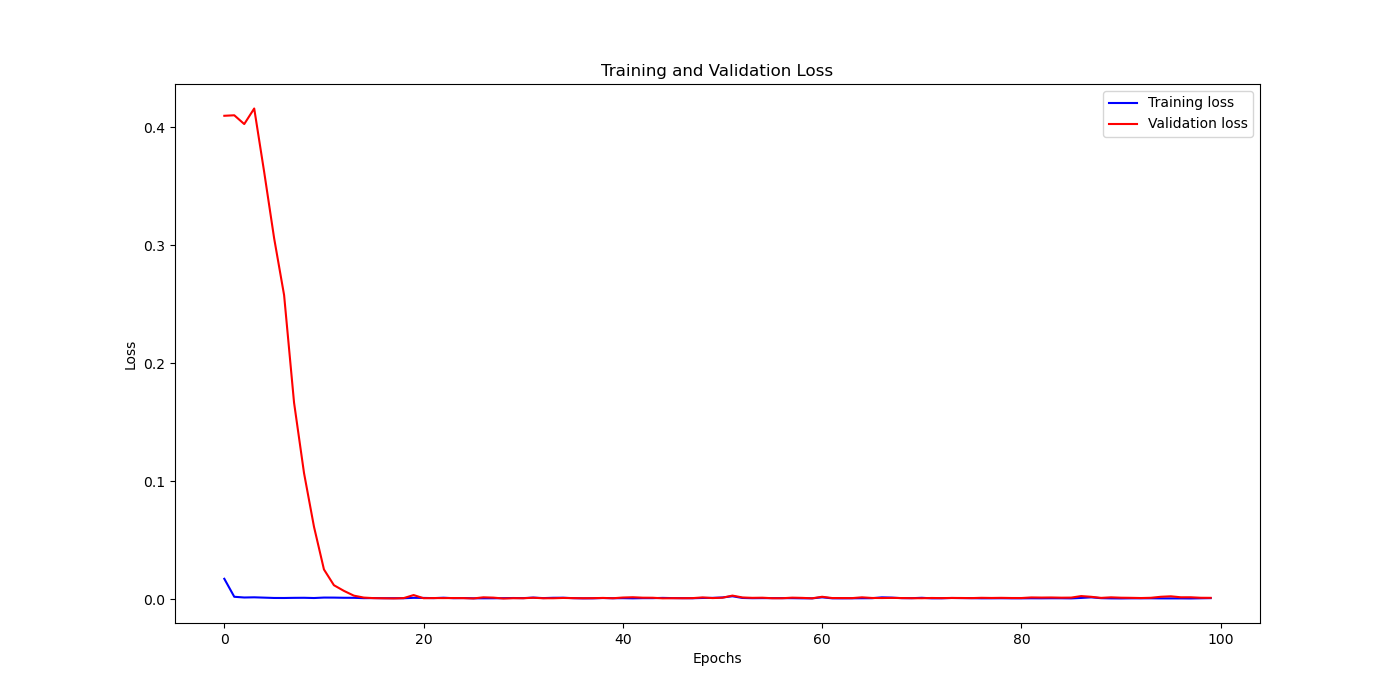
\includegraphics[width=\textwidth]{manuscript/src/figures/Ass4/Ass4_Q2c_Training and Validation Loss.png}
    \end{minipage}
    \caption{Training and Validation Loss of model (c) versus epoch..}
    \label{fig:Ass4_Q2c_Training}
\end{figure}












